%!TEX root = ../main.tex

\newpage

\section{Préparation de l'environnement}
Dans cette section, l'environnement et les outils nécessaire pour le bon fonctionnement du projet seront installer
et préparé correctement. Il y en a en gros trois machines différentes : une machine d'attaque, une machine vulnérable,
et finalement une machine sécurisé.

    \subsubsection{La machine d'attaque} 
    Cette machine sera équiper du système d'exploitation \emph{Kali Linux \cite{linux} Rolling} (figure ), le 
    leader des systèmes de testes d'intrusions. Après le téléchargement de l'image
    ISO depuis le site officiel de Kali, et l'installation de l'image sur
    une machine virtuelle, une mise à jours complète du système est faite par le biais de cette commande : 
    ``\texttt{sudo apt-get update \&\& sudo apt-get upgrade}'' (Pour une explication des commandes utilisées,
    consultez \autoref{commandes}).
        \begin{center}
            photo de kali linux avec la commande ``sudo apt-get update \&\& sudo apt-get upgrade''
        \end{center}

    \subsubsection{La machine vulnérable} \label{machine_vulnerable} 
    Cette machine sera équiper d'une version \emph{Windows 7}  
    doté d'un service vulnérable et d'un pare-feu désactiver. Le service vulnérable installé sur cette 
    machine est un service \emph{ftp} manipulé par le programme \emph{KONICA MINOLTA FTP Utility} 
    (\autoref{la_machine_vulnerable}).
    \begin{figure}[h!]
        \centering
        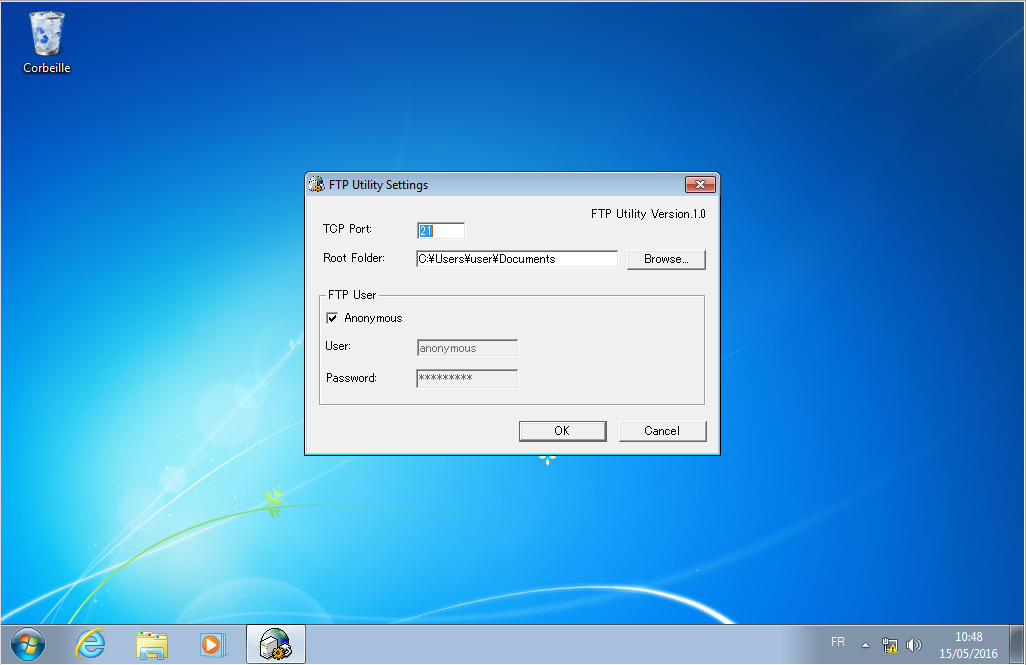
\includegraphics[scale=0.3]{images/Windows_7_2.png}
        \caption{La machine vulnérable}
        \label{la_machine_vulnerable}
    \end{figure}

    \subsubsection{La machine sécurisé} 
    Cette machine sera équiper de \emph{Windows 7} avec un anti virus et un pare-feu fonctionnel.

\subsection{Réseau}
    Les trois machines seront dans le réseau \cite{reseau} dont l'adresse est \emph{172.16.178.0/24}. 
    La machine d'attaque aura l'adresse IP \emph{172.16.178.1} ; la machine vulnérable aura l'adresse IP 
    \emph{172.16.178.129} ; et finalement, la machine sécurisé aura l'adresse IP \emph{172.16.172.130}.

    Pour voir comment le réseau a été configuré sur chaque machine, consultez \autoref{config_reseau}.


\section{Développement}
    \subsection{Backdoor}
    \subsection{Virus infecteur}
    La méthode d’infection que nous allons utiliser est : l’injection de code dans un exécutable par \emph{Ajout}
    dont une définition claire a été abordée dans le chapitre précédent.

    Cette technique, se base sur la manipulation de la structure PE (une définition détaillée a été donnée dans le 
    \autoref{pe_header}), nous avons donc inclus la bibliothèque \emph{Windows.h} qui contient les 
    structures et fonctions nécessaires.

    Le code se divise en deux fonctions primordiales :
    \begin{description}
        \item[WinMain :] Cette fonction est la fonction Main, dans un premier temps son rôle est de créer 
        deux espaces mémoire pour y stocker le code du Virus et du Backdoor, puis de cibler un exécutable. 
        une vérification sera faite sur sa compatibilité avec Windows 32 bits.

        Dans un deuxième temps, elle ouvre ce dernier et récupère sa structure PE. Après des calculs précis, 
        elle stocke dans une variable le Point d’Entrer Original appelé \emph{OEP} et ajoute à la fin de ce 
        fichier deux nouveaux segments; le segment qui contient le code du Virus et un autre qui contient 
        le code du Backdoor puis les crypte avec une clé prédéfinie. A la fin, elle 
        change le point d’entrer et le fait pointer vers la fonction VirusCode (\autoref{changement_point_entree}).
        La fonction modifie aussi le \emph{loader flags}\footnote{\emph{loader flags} est un flag obsolète non
        utiliser par Windows.} et y place notre flag d'infection. En dernier, une correction du \emph{Checksum}
        sera faite.
        
        \item[VirusCode :] Cette fonction sera le nouveau point d’enter de chaque exécutable infecté, 
            elle s’exécutera toujours en premier puis elle donnera la main au code original, 
            elle passe par trois étapes clé : \\
            Premièrement, une récupération de l'adresse de la bibliothèque Kernel32 chargé avec l'exécutable 
            hôte est primordiale pour trouver et stocker les adresses des fonctions  nécessaires au bon 
            fonctionnement du code malveillant.
            deuxièmement, elle chargera l’adresse du segment du Virus et du Backdoor, créera deux 
            emplacements mémoire et les copie dedans, puis elle les décrypte.
            Et enfin, elle créera deux fichiers exécutables dans le dossier “temp”, un contenant le Virus et 
            l’autre le Backdoor, et les exécutera. En dernier, un appel vers le point d’entrer original sera fait.

    \end{description}

    \begin{figure}[h]
        \centering
        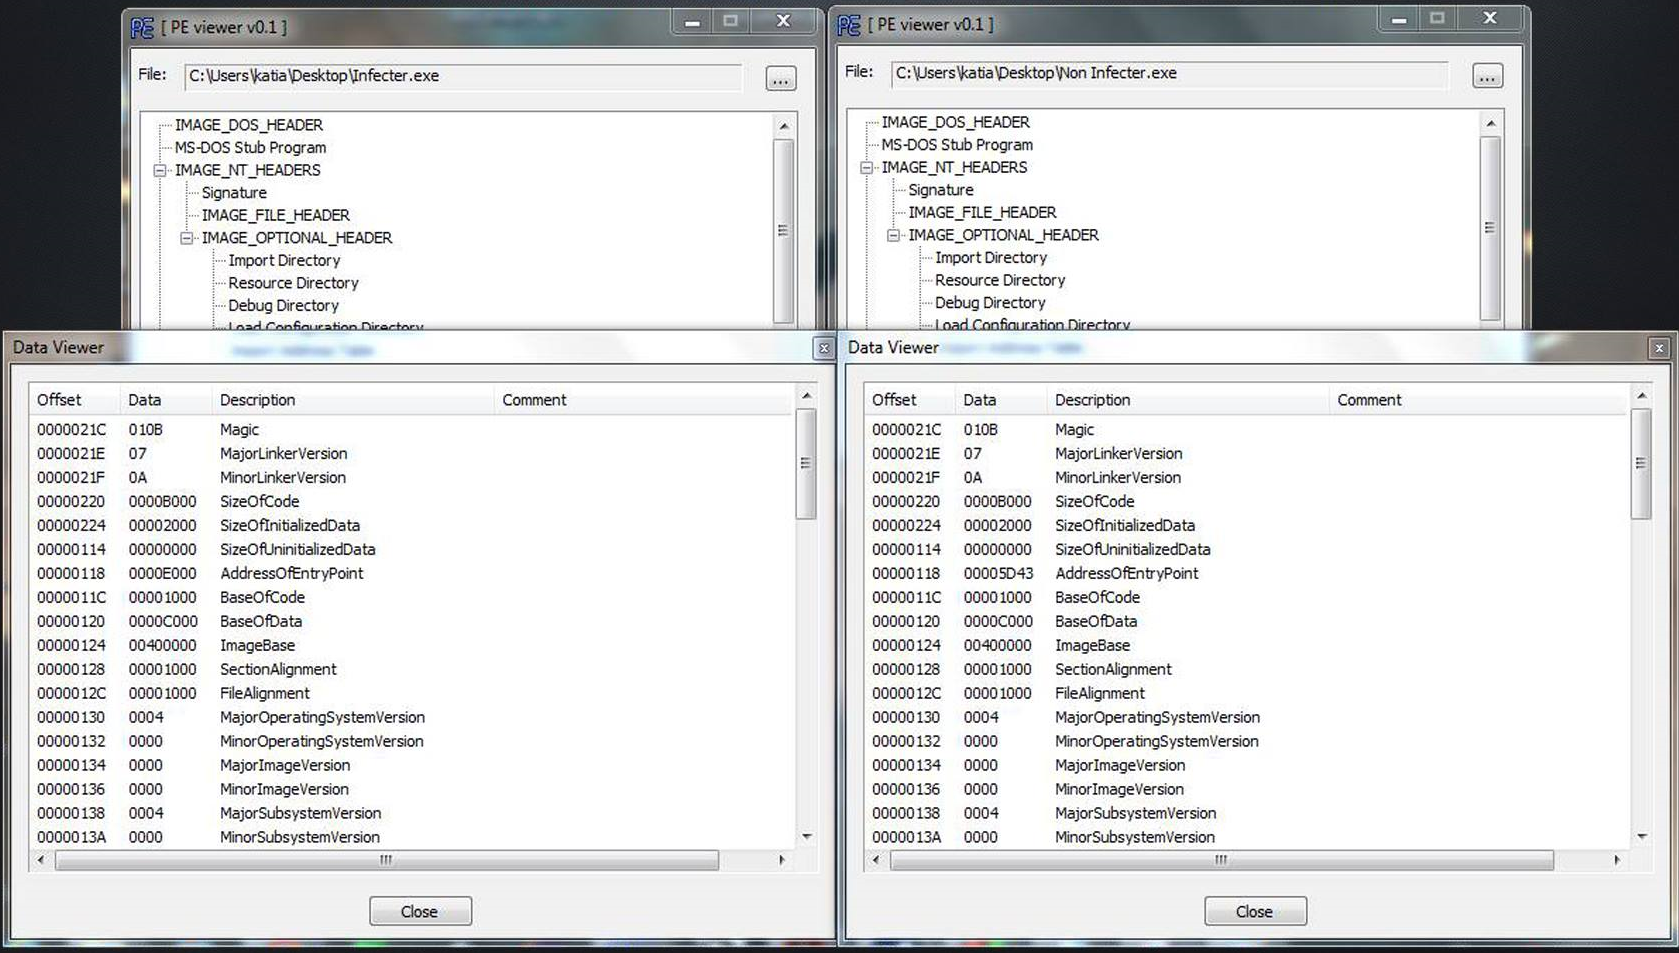
\includegraphics[width=\linewidth]{images/pe_changes.png}
        \caption{Changement du point d'entré}
        \label{changement_point_entree}
    \end{figure}

    Nous citerons aussi que ce Virus infecte les fichiers exécutables des clés USB connecté à la machine.
    La particularité majeure de notre Virus est qu’il utilise des API native, et qu’il ne peut pas être 
    déboguer, une démonstration est montrer dans la figure suivante:

\section{Exploitation}
Cette section sera consacré à l'exploitation de la machine vulnérable, et l'obtention d'un accès à distance
sur cette dernière. On commencera par une bref présentation des outils utilisés pour une meilleur compréhension
de cette section.
    \subsection{Présentation des outils}
    \begin{description}
        \item[netcat :] C'est un outil utilisé en ligne de commande, et qui permet l'ouverture des connexions
            réseau, que ce soit \emph{TCP} \cite{reseau} ou \emph{UDP} \cite{reseau}. En raison de sa polyvalence,
            il est aussi appelé le \emph{couteau suisse} du réseau.

            Pour se connecter à un serveur sur un port donnée, il faut donner à \emph{netcat} deux paramètres qui sont 
            l'adresse du serveur et le port qu'utilise le serveur. Exemple :
            \begin{lstlisting}[language=bash] 
            $ netcat www.google.com 80
            \end{lstlisting}

            Dans le côté serveur, pour mettre netcat en écoute sur un port, il faut préciser deux options qui sont 
            `\emph{-l}' pour dire à netcat d'écouter, et `\emph{-p \ul{port}}' pour préciser le port d'écoute.
            Exemple :
            \begin{lstlisting}
            # netcat -l -p 80   
            \end{lstlisting}

        \item[Metasploit :] C'est un \emph{Framework} de testes de pénétrations \emph{open source} utilisé pour 
            tester la robustesse des machines en matière de sécurité. Il est composé essentiellement de charges 
            et d'exploits. 

        \item[msfvenom :] \label{msfvenom} C'est un générateur et encodeurs de charges. Il est utile pour une utilisation plus manuelle
            des charges, car il permet de générer ces dernières dans plusieurs format (des exécutables, pour un 
            script python \ldots{}). 

            Plusieurs paramètres sont à utiliser pour obtenir des charges plus performantes. Parmi ces options on y
            trouve :
            \begin{description}
                \item[-a \ul{architecture} :] L'architecture du système dont la charge est destiné
                    (x86 ou x64).
                \item[--plateform \ul{plateforme} :] Le système attaqué (Windows, Mac, Linux, Android
                \ldots{}).
                \item[-p \ul{charge} \ul{options\_de\_la\_charge}:] La charge et les options utilisés 
                    pour générer celle-ci.
                \item[-e \ul{encodage} :] L'encodage utilisé pour générer la charge.
                \item[-b \ul{mauvais\_octets} :] Les octets à éviter pendant la génération de la charge.
                \item[-f \ul{format} :] Format de la charge (exécutable, python, perl \ldots{}).
            \end{description}

        \item[meterpreter :] \label{meterpreter}C'est une charge avancée et extensible développé par les développeurs de 
            \emph{Metasploit}. Elle est utilisé par ce dernier pour donner un accès plus étendu et plus 
            complet à une machine exploitable. 
    \end{description}

    \subsection{La vulnérabilité}
    Le service vulnérable qui a été installé est un service \emph{ftp} manipulé par le programme 
    \emph{Konica Minolta FTP Utility}. 
    La vulnérabilité découverte, qui est un débordement de tampon (\autoref{buffer_overflow}), a été publié le 11
    Janvier 2016 sur le site d'\emph{Exploit Database}\footnote{\emph{Exploit Database} est un site qui se charge
    d'archiver les exploits publics et les logiciels vulnérables correspondants. Ce site dont le lien est 
    \url{www.exploit-db.com} est développé par les testeurs d'intrusions et les chercheurs de vulnérabilités.}.

    La version vulnérable du programme peut être obtenu depuis ce lien 
    \url{https://www.exploit-db.com/apps/6388a2ae7dd2965225b3c8fad62f2b3b-ftpu_10.zip}.

    \subsection{L'exploit}
    Le script qui permet d'exploiter cette vulnérabilité peut être récupérer depuis ce lien 
    \url{https://www.exploit-db.com/exploits/39215/}.
    Ce script \emph{python} se divise en deux parties :
    \begin{description}
        \item[Exploit :] Cette partie du script permet en quelque sorte de préparer le programme vulnérable à 
            recevoir le code malveillant pour l'exécution. Cette partie n'est pas à modifier, car elle a été développé
            après une étude approfondie du programme vulnérable.

        \item[Charge :] Cette partie du script représente le code qui sera exécuté sur l'application vulnérable. 
            Cette partie peut être remplacé par la charge désiré par l'attaquant.
            % L'exploit téléchargé depuis ce lien \url{https://www.exploit-db.com/exploits/39215/} vient avec une charge
            % par défaut, qui est un \emph{reverse shell}.% Pour notre démonstration, on ne va pas utiliser 
            % la charge par défaut, mais on va plutôt utiliser une autre charge qui permet d'exécuter un programme 
            % beaucoup plus puissant, qui est \emph{meterpreter}. 
    \end{description}

    Le script va se connecter à la machine victime sur le port 21 (\autoref{execution_script_exploitation}). 
    La charge qu'utilise le 
    script va ordonné à la machine qu'elle donne un reverse shell en se reconnectant à la machine de l'attaquant 
    sur le port 4444. Pour intercepter ce reverse shell, et pouvoir communiquer avec
    la machine victime, il faut ordonner à netcat d'écouter sur le port 4444 (\autoref{obtention_reverse_shell}).

    \begin{figure}[h!]
        \centering
        \begin{subfigure}{0.9\textwidth}
            \centering
            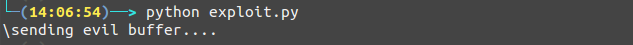
\includegraphics[width=\textwidth]{images/exploit_python.png}
            \caption{Exécution du script d'exploitation}
            \label{execution_script_exploitation}
        \end{subfigure}
        \hfill
        \begin{subfigure}{0.9\textwidth}
            \centering
            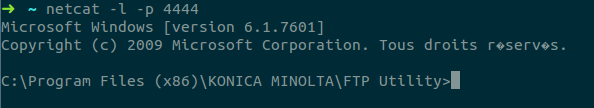
\includegraphics[width=\textwidth]{images/reverse_shell.png}
            \caption{Obtention du reverse shell}
            \label{obtention_reverse_shell}
        \end{subfigure}
        \hfill
        \caption{Exploitation avec la charge d'origine}
        \label{exploitation_avec_charge_origine}
    \end{figure}

    La charge par défaut de ce script est une charge un petit peu limitée, donc nous allons nous en servir 
    de \emph{msfvenom} pour générer la charge \emph{meterpreter} (\autoref{generation_charge}) et l'utiliser 
    dans le script d'exploitation.
    \begin{figure}[h]
        \centering
        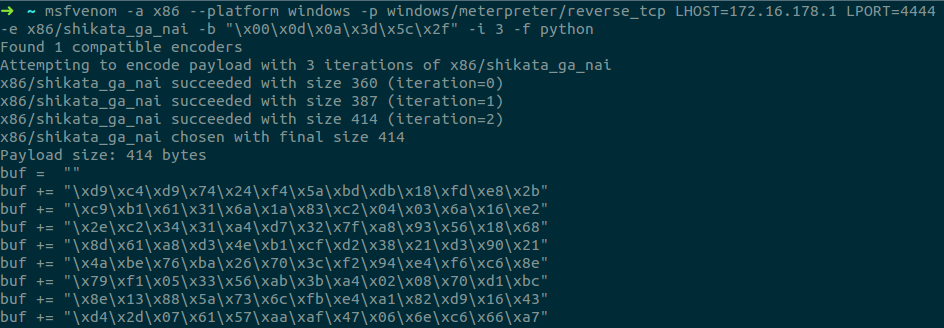
\includegraphics[width=\linewidth]{images/msfvenom.png}
        \caption{Génération de la charge}
        \label{generation_charge}
    \end{figure}

    \subsection{Obtention d'accès}
    Pour la charge utilisé précédemment, il a suffit d'utiliser netcat pour intercepter la connexion et communiquer
    avec la machine victime. Mais meterpreter exige des techniques plus poussées pour pouvoir faire cela, 
    donc nous allons faire appel aux services de Metasploit pour accomplir cette tâche.
    On commence par lancer Metasploit en mode console (\autoref{msfconsole}) par le biais de la commande 
    `\emph{msfconsole}'. Après, on effectue les manipulations nécessaires (\autoref{config_metasploit})
    pour pouvoir intercepter les réponses de meterpreter.

    \begin{figure}[h!t]
        \centering
        \begin{subfigure}{0.9\textwidth}
            \centering
            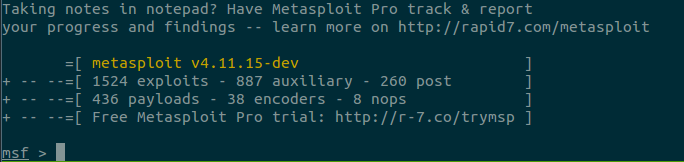
\includegraphics[width=\textwidth]{images/msfconsole.png}
            \caption{Lancement de Metasploit}
            \label{msfconsole}
        \end{subfigure}
        \hfill
        \begin{subfigure}{0.9\textwidth}
            \centering
            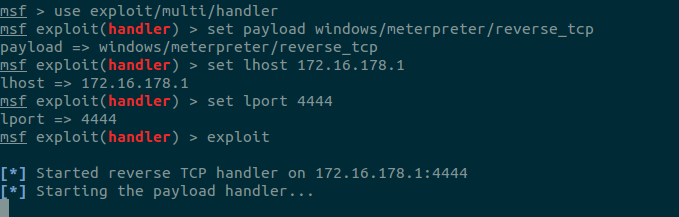
\includegraphics[width=\textwidth]{images/ecoute_msf.png}
            \caption{Configuration de Metasploit}
            \label{config_metasploit}
        \end{subfigure}
        \hfill
        \caption{Préparation de Metasploit}
        \label{exploitation_avec_charge_origine}
    \end{figure}

    Maintenant, il ne reste plus qu'à lancer le script d'exploitation qu'on a modifié et obtenir un accès à la 
    machine exploité (\autoref{obtention_accees_meterpreter}).

    \begin{figure}[h!t]
        \centering
        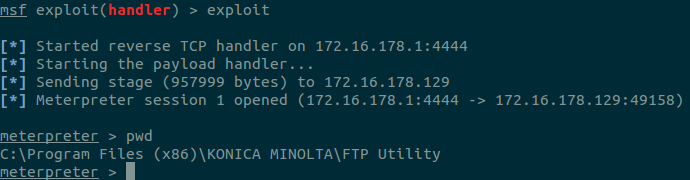
\includegraphics[width=\linewidth]{images/meterpreter.png}
        \caption{Obtention de l'accès avec meterpreter}
        \label{obtention_accees_meterpreter}
    \end{figure}

\section{Teste de propagation}
\section{Conclusion}
